\documentclass[11pt]{article}
\usepackage{etoolbox}
\usepackage[letterpaper,margin=1in]{geometry}
\usepackage[parfill]{parskip}
\usepackage{amsmath,amssymb,graphicx}
\usepackage{fancyhdr}
\usepackage{enumerate}
\usepackage{xcolor}
\usepackage{cancel}
\usepackage{tikz}


\newcommand{\sol}{\bigskip\textbf{Solution.}\qquad\qquad}

\setlength{\headheight}{14pt}
\renewcommand{\baselinestretch}{1.3}
\pagestyle{fancyplain}
\fancyfoot{}
\fancyhead[L]{Exam \HomeworkNo{}}
\fancyhead[C]{OMCIT 592}
\fancyhead[R]{\thepage}
\renewcommand{\headrulewidth}{0pt}
\setlength{\headheight}{14pt}
\setlength{\headsep}{12pt}
\setlength{\footskip}{0pt}

\fancypagestyle{firstpage}{
  \fancyhead{}
  \fancyfoot{}
}


\newcommand{\problembreak}{\bigskip\hrule\bigskip}
\newcommand{\points}[1]{\textbf{[#1 pts]}}


\newcommand{\HomeworkNo}{3}


\begin{document}
\thispagestyle{firstpage}
\begin{center}
{\Large OMCIT 592 Spring 2022 \hfill Timed Exam \HomeworkNo}\\[20pt]

%%%%%%%%%%%%%%%%%%%%%%%%%%%%%%%%%%%%%%
%%%  DO NOT MODIFY ABOVE THIS LINE  %%
%%%%%%%%%%%%%%%%%%%%%%%%%%%%%%%%%%%%%%


%%%%%%%%%%%%%%%%%%%%%%%%%%%%%%%%%%%%%%%%%%%%%%%%%%%%%%%%%%%%%%%%%%%%%%%%%%%%%%%%%%%%%%%%%%%%%%
%%%    USEFUL RESOURCES BELOW (you can copy and paste these resources to your solutions)   %%%
%%%%%%%%%%%%%%%%%%%%%%%%%%%%%%%%%%%%%%%%%%%%%%%%%%%%%%%%%%%%%%%%%%%%%%%%%%%%%%%%%%%%%%%%%%%%%%

% 1. Fraction x/y
% \frac{x}{y}

% 2. Square root (\sqrt{x}), Logarithm with base b (\log_b{x}), Natural Log (\ln{x}) 

% 3. Binomial n Choose k
% \binom{n}{k}

% 4. Greater than or equal (\geq}, less than or equal (\leq), not equal (\neq) commands 

% 5. Logical or (\lor or \vee), logical and (\land or \wedge), logical implication (\implies),  logical negation (\neq), and logical equivalence (\equiv) commands. 

% 6. Set union (\cup), set intersection (\cap), empty set \emptyset, strict subset (\subset), strict super-set (\supset), not necessarily proper/strict subset (\subseteq), not necessarily proper/strict super-set (\supseteq) 

%7. Probabilities: Pr[A] (\Pr[A]), Expectation E[X] (\E[X])

%8. Dots ... (\ldots)

%9. Box Correct answer \boxed{answer}

%10. Dot Product • (\cdot)

%11. Perpendicular/Independent (\perp), Not Independent (\not\perp)

%12. Undirected edge u-v   Directed edge u\rightarrow v

%13. Undirected walk/path  u-\cdots-v  Directed walk/path  u \twoheadrightarrow v

%%%%%%%%%%%%%%%%%%%%%%%%%%%%%%%%%%%%%%%%%%%%%%%%%%%%%%%
%%%    COMPLETE EMAIL AND NAME IN FIELDS BELOW      %%%
%%%%%%%%%%%%%%%%%%%%%%%%%%%%%%%%%%%%%%%%%%%%%%%%%%%%%%%


YOUR NAME
\hfill
YOUR PENN EMAIL ADDRESS
\hfill
\today
\end{center}

\vspace*{1cm}


%%%%%%%%%%%%%%%%%%%%%%%%%%%%%%%%%%%%%%
%%%  DO NOT MODIFY BETWEEN THESE LINES%%
%%%%%%%%%%%%%%%%%%%%%%%%%%%%%%%%%%%%%%


\rule{\textwidth}{0.4pt}
\begin{quote}
To receive full
credit all your answers should be carefully justified.
Each solution must be written independently by yourself - \textbf{no collaboration is allowed}.
\end{quote}
\rule{\textwidth}{0.4pt}

\textsc{Six (6) Problems for a Total of 60 Points}


%%%%%%%%%%%%%%%%%%%%%%%%%%%%%%%%%%%%%%
%%%  DO NOT MODIFY BETWEEN THESE LINES  %%
%%%%%%%%%%%%%%%%%%%%%%%%%%%%%%%%%%%%%%


Below, \emph{graph} always refers to an undirected graph; directed graphs are called digraphs.
\begin{enumerate}

%%%%%%%%%%%%%%%%%%%%
%%%  PROBLEM 1  %%%
%%%%%%%%%%%%%%%%%%%%
	\item {[10pts]}
	By determining which vertices should be red, green, and blue, give a proper 3-coloring of the graph below. Your answer should consist of three lists: a list
	of the red vertices, a list of the green vertices, and a list of the blue vertices. You are not required to draw anything in your answer.
	
		\begin{center}
		\begin{tikzpicture}[scale=0.5]
		\tikzstyle{every node}+=[draw,thick,circle,inner sep=0pt,minimum size=20]
		\node (a) at (0.5,1)  {$7$};
		\node (b) at (3.5,1)  {$8$};
		\node (c) at (4.5,3.5)  {$6$};
		\node (d) at (2,5.5) {$5$};
		\node (e) at (-0.5,3.5)  {$4$};
		\node (f) at (-1.5,-1)  {$9$};
		\node (g) at (5.5,-1) {$10$};
		\node (h) at (7,4.5) {$3$};
		\node (i) at (2,8) {$2$};
		\node (j) at (-3,4.5)  {$1$};
		\tikzstyle{every edge}+=[thick]
		\draw (a) edge (b) edge (f)
			  (b) edge (c) edge (g)
			  (c) edge (d) edge (h)
			  (d) edge (e) edge (i)
			  (e) edge (a) edge (j)
			  (f) edge (g)
			  (g) edge (h)
			  (h) edge (i)
			  (i) edge (j)
			  (j) edge (f);
		\end{tikzpicture}
		
	\end{center}
    
\textbf{Solution.} \\
	YOUR SOLUTION GOES HERE
	
	
	~\\~\\
	
%%%%%%%%%%%%%%%%%%%%
%%%  PROBLEM 2  %%%
%%%%%%%%%%%%%%%%%%%%
	
		\item {[10pts]}
		Topologically sort the vertices of the digraph below. Your answer should be a sequence (list) of vertices that forms a topological sort. You are not required to draw anything in your answer.
	
	\begin{center}
		\begin{tikzpicture}[scale=0.5]
		\tikzstyle{every node}+=[draw,thick,circle,inner sep=0pt,minimum size=20]
		\node (a) at (0.5,1)  {$a$};
		\node (b) at (3.5,1)  {$b$};
		\node (c) at (4.5,3.5)  {$c$};
		\node (d) at (2,5.5) {$d$};
		\node (e) at (-0.5,3.5)  {$e$};
		\node (f) at (-1.5,-1)  {$f$};
		\node (g) at (5.5,-1) {$g$};
		\node (h) at (7,4.5) {$h$};
		\node (i) at (2,8) {$i$};
		\node (j) at (-3,4.5)  {$j$};
		\tikzstyle{every edge}+=[->,thick]
		\draw (a) edge (b) edge (e) edge (f)
		(b) edge (c)
		(c) edge (d) edge (h)
		(d) edge (e) edge (i)
		(e) edge (j)
		(f) edge (g) edge (j)
		(g) edge (h) edge (b)
		(i) edge (h) edge (j);
		\end{tikzpicture}
		
	\end{center}
    
\textbf{Solution.} \\
	YOUR SOLUTION GOES HERE
	
	~\\~\\
	
%%%%%%%%%%%%%%%%%%%%
%%%  PROBLEM 3  %%%
%%%%%%%%%%%%%%%%%%%%
	
	
	\item {[10pts]}
	What are the strongly connected components of the digraph below?
	Your answer should consist of a list of strongly connected components
	where each component is represented as a set of vertices. You are not required to draw anything in your answer.
	
	\begin{center}
	\begin{tikzpicture}[scale=0.75]
		\tikzstyle{every node}+=[draw,thick,circle,inner sep=0pt,minimum size=20]
		\node (a) at (0,0)  {$4$};
		\node (b) at (0,3)  {$5$};
		\node (c) at (2,5)  {$7$};
		\node (d) at (4,3) {$9$};
		\node (e) at (4,0)  {$8$};
		\node (f) at (2,2)  {$6$};
		\node (g) at (6,0) {$10$};
		\node (h) at (6,5) {$11$};
		\node (i) at (-2,5) {$2$};
		\node (j) at (-2,0)  {$3$};
		\node (k) at (-4,2) {$1$};
		\node (l) at (8,2) {$12$};
		\tikzstyle{every edge}+=[->,thick]
		\draw
		(a) edge (f) edge (j)
		(b) edge (f)
		(c) edge (b)
		(d) edge (h)
		(e) edge (d)
		(f) edge (d) edge (c)
		(g) edge (l)
		(h) edge (l) edge (c)
		(i) edge (a) edge (c)
		(j) edge (k)
		(k) edge (i)
		;
		\draw[bend left=20]
		(e) edge (g)
		(g) edge (e)
		;
	\end{tikzpicture}
	
	\end{center}
	
\textbf{Solution.} \\
	YOUR SOLUTION GOES HERE
	
	~\\~\\
	
%%%%%%%%%%%%%%%%%%%%
%%%  PROBLEM 4  %%%
%%%%%%%%%%%%%%%%%%%%
	
\item {[10pts]} Let $G=(V,E)$ be a connected graph in which every vertex is a leaf. 
Prove that $G$ has exactly one edge. You are not required to draw anything in your proof.


\textbf{Solution.} \\
	YOUR SOLUTION GOES HERE
	
	~\\~\\
	
%%%%%%%%%%%%%%%%%%%%
%%%  PROBLEM 5  %%%
%%%%%%%%%%%%%%%%%%%%
	
\item {[15pts]}
Let $G=(V,E)$ be a digraph in which every vertex is a source, or a sink, or both a sink and a source.
\begin{enumerate}
    \item {[7pts]} Prove that $G$ has neither self-loops nor anti-parallel edges.
    \item {[8pts]} Let $G^u=(V,E^u)$ be the undirected graph obtained by erasing the direction on the edges of $G$. Prove that $G^u$ has chromatic number 1 or 2.
\end{enumerate}
You are not required to draw anything in your proofs.
	
	
\textbf{Solution.} \\
\begin{enumerate}
    \item {[7pts]} YOUR SOLUTION TO PART (a) HERE
    \item {[8pts]} YOUR SOLUTION TO PART (b) HERE
\end{enumerate}

	~\\~\\
	
%%%%%%%%%%%%%%%%%%%%
%%%  PROBLEM 6  %%%
%%%%%%%%%%%%%%%%%%%%
	
\item {[5pts]} Let $G=(V,E)$ be a graph such that
	\begin{itemize}
	    \item $|V|\geq 3$, 
	    \item $G$ has exactly 2 leaves, and
	    \item in $G$ all the non-leaf vertices have degree 3 or more.
	\end{itemize}
	Prove that $G$ has at least one cycle. You are not required to draw anything in your proof.
	
	
\textbf{Solution.} \\
	YOUR SOLUTION GOES HERE
	
	~\\~\\
	
	
\end{enumerate}
\end{document}